\section{The Ladder \protect
\includegraphics[height=1em]{figs/ladder.png}: Agent improvement with AutoLibra}
\label{sec:ladder}

In this section, we use AutoLibra to iteratively improve agent performance (as a 'ladder') through prompt engineering and fine-tuning, to comprehensively study whether the induced metrics are good optimization targets. 
%On a text-game task (Baba-Is-AI), \diyi{delete this sentence of results and use the following subsections to share about your results, to avoid repetition. } we find that optimizing prompts driven by iteratively induced metrics improves the performance of state-of-the-art agents significantly. Similarly, on web navigation tasks, we find that fine-tuning on the data selected by the induced metrics can iteratively improve the agent performance better than goal-oriented scores. 
Fig. \ref{fig:autolibra-training} illustrates the results. In all experiments, GPT-4o is used as (at the time of writing) it has a leading bench on the BALROG benchmark \cite{paglieri2024balrog}; Claude-3.5-Sonnet is used in ablations as it has a comparable bench (32.3 \% vs. 32.6 \%), respectively.

\subsection{Agent prompt engineering case study: Baba-Is-AI}
\label{sec:Baba-Is-AI}

Baba-Is-AI \citep{cloos2024babaaibreakrules} is a grid world game which is especially challenging for LLM agents since it requires navigation and interaction with blocks that modify in-environment rules. Implementation-specific details are discussed in more detail in Appendix \ref{appendix:baba_is_ai_rules}.


% \begin{figure}[ht]
%     \centering
%     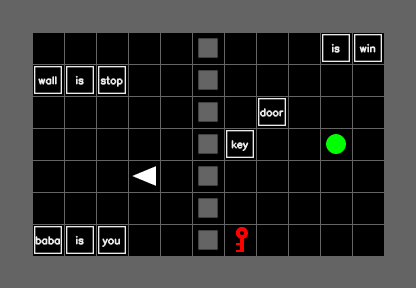
\includegraphics[scale=0.5]{figs/babaisai_env.png}
%     \caption{Example of the Baba-Is-AI environment. In this task (two\_room-break\_stop-make\_win-distr\_obj-irrelevant\_rule), the agent has to break the "wall is stop" rule and push the "key" rule block next to "is win" to assemble the win rule, then touch the key to win. Pushing the "door" rule block would be a mistake, as no door object is present.}
%     \label{fig:babaisai_env}
% \end{figure}

% \subsection{AutoLibra for Baba-Is-AI improvement}


In performing iterative agent improvement with AutoLibra, a full cycle of the AutoLibra ladder pipeline is considered one \textit{Iteration}, for which the pseudocode and environment configuration are detailed in Appendix \ref{appendix:algo1}.

\begin{wraptable}[19]{r}{0.60\textwidth} % 'r' for right, adjust the width as needed
\centering
\small
\vspace{-30pt}
\begin{tabular}{ccl}
\toprule
\multicolumn{1}{c}{Emoji}& 
\multicolumn{1}{c}{It.} & 
\multicolumn{1}{l}{Metric} \\
\midrule
\rowcolor{gray!10} 
\includegraphics[scale=0.07]{figs/emojis/emoji_1.png} & 0 & Win Condition Recognition \\
\midrule
\rowcolor{gray!10} 
\includegraphics[scale=0.07]{figs/emojis/emoji_2.png} & 0 & Rule Modification \\
\midrule
\rowcolor{gray!10} 
\includegraphics[scale=0.07]{figs/emojis/emoji_3.png} & 0 & Direct Navigation Efficiency \\
\midrule
\rowcolor{gray!10} 
\includegraphics[scale=0.07]{figs/emojis/emoji_4.png} & 0 & Context-Sensitive Decision Making \\
\midrule
\rowcolor{gray!30} 
\includegraphics[scale=0.07]{figs/emojis/emoji_5.png} & 1 & Win Rule Construction \\
\midrule
\rowcolor{gray!30} 
\includegraphics[scale=0.07]{figs/emojis/emoji_6.png} & 1 & Selective Interaction With Relevant Objects  \\
\midrule
\rowcolor{gray!30} 
\includegraphics[scale=0.07]{figs/emojis/emoji_7.png} & 1 & Rule Manipulation and Execution  \\
\midrule
\rowcolor{gray!60} 
\includegraphics[scale=0.07]{figs/emojis/emoji_8.png} & 2 & Subtask Coordination \\
\midrule
\rowcolor{gray!90} 
\includegraphics[scale=0.07]{figs/emojis/emoji_9.png} & 3 & Immovable Interaction \\
\bottomrule
\end{tabular}
\caption{Metrics and Turn of Induction \newline for Baba-Is-AI}
\label{tab:metrics}
\end{wraptable}

% \begin{figure}[ht]
%     \centering
%     \begin{minipage} % First table in a minipage taking 45% of the text width
%         \begin{wraptable}[19]{r}{0.60\textwidth} % 'r' for right, adjust the width as needed
\centering
\small
\vspace{-30pt}
\begin{tabular}{ccl}
\toprule
\multicolumn{1}{c}{Emoji}& 
\multicolumn{1}{c}{It.} & 
\multicolumn{1}{l}{Metric} \\
\midrule
\rowcolor{gray!10} 
\includegraphics[scale=0.07]{figs/emojis/emoji_1.png} & 0 & Win Condition Recognition \\
\midrule
\rowcolor{gray!10} 
\includegraphics[scale=0.07]{figs/emojis/emoji_2.png} & 0 & Rule Modification \\
\midrule
\rowcolor{gray!10} 
\includegraphics[scale=0.07]{figs/emojis/emoji_3.png} & 0 & Direct Navigation Efficiency \\
\midrule
\rowcolor{gray!10} 
\includegraphics[scale=0.07]{figs/emojis/emoji_4.png} & 0 & Context-Sensitive Decision Making \\
\midrule
\rowcolor{gray!30} 
\includegraphics[scale=0.07]{figs/emojis/emoji_5.png} & 1 & Win Rule Construction \\
\midrule
\rowcolor{gray!30} 
\includegraphics[scale=0.07]{figs/emojis/emoji_6.png} & 1 & Selective Interaction With Relevant Objects  \\
\midrule
\rowcolor{gray!30} 
\includegraphics[scale=0.07]{figs/emojis/emoji_7.png} & 1 & Rule Manipulation and Execution  \\
\midrule
\rowcolor{gray!60} 
\includegraphics[scale=0.07]{figs/emojis/emoji_8.png} & 2 & Subtask Coordination \\
\midrule
\rowcolor{gray!90} 
\includegraphics[scale=0.07]{figs/emojis/emoji_9.png} & 3 & Immovable Interaction \\
\bottomrule
\end{tabular}
\caption{Metrics and Turn of Induction \newline for Baba-Is-AI}
\label{tab:metrics}
\end{wraptable} % Your first table
%     \end{minipage}%
%     \hfill % Adds some horizontal space between the tables
%     \begin{minipage} % Second table in a minipage taking 45% of the text width
%         \centering
%         \renewcommand{\arraystretch}{1.5} 
\begin{table}[h!]

\centering
\begin{tabular}{|>{\raggedright\arraybackslash}p{6cm}|c|c|c|c|}
\hline
\textbf{Turn} & \textbf{0} & \textbf{1} & \textbf{2} & \textbf{3} \\
\hline
\textbf{Babaisai Score GPT-4o} & 0.30 & 0.40 & 0.43 & 0.55 \\
\hline
\textbf{Babaisai Score Claude 3.5 Sonnet} & 0.35 & 0.40 & 0.45 & 0.55 \\
\hline
\textbf{Average Env. Steps} & 79 & 63 & 60 & 51 \\
\hline
\end{tabular}
\caption{Babaisai Scores and Average Environment Steps}
\end{table} % Your second table
%     \end{minipage}
%     \caption{Tables side by side}
% \end{figure}

\paragraph{Results}

Held-out task performance increased by 25\% to 55\% between \textit{Iteration 0} and \textit{Iteration 3}, with each iteration resulting in greater performance than the last (Full held-out task results tabulated in Appendix \ref{appendix:heldout}); \textbf{this result was replicated across several tested models}. This represents a substantial increase compared to the highest base model performance of 33\% on Baba-Is-AI \citep{paglieri2024balrog}, demonstrating that improvements realized by AutoLibra are generalizable to unseen tasks and validating the utility of the framework in augmenting the performance of agents in highly diverse environments. Among induced metrics (Table \ref{tab:metrics}), agent performance increases correspondingly to code changes targeting those metrics, an example being \texttt{Win Condition Recognition} 
\includegraphics[scale=0.07]{figs/emojis/emoji_1.png}, which increases from 28\% to 50\% from \textit{Iterations 0-1} after few-shot prompting is introduced to demonstrate identifying a win condition rule, with a full list of improvements and examples presented in Appendix \ref{appendix:baba_is_ai_obs}. The high correlation between induced metrics, targeted changes to agent code, and improvements in the agent performance on those metrics validates the fine-grainedness and human-interpretability of AutoLibra metrics, and demonstrates its utility in targeted improvement of agent behaviors.

Similarly to results observed in Section 3, induced metrics are observed to capture the behavior of the agent increasingly well with additional iterations, with coverage increasing from 65\% at \textit{Iteration 0} to 92\% at \textit{Iteration}, while mean redundancy remains 56\% across all iterations. The trajectory performance also improved significantly, with the average number of steps per task (capped at 100) decreasing from 79 to 51, indicating that the agent's reasoning performance and efficiency improved as a result of the code changes made in each iteration.

Qualitative observation of agent trajectories reveals behaviors commensurate with induced metric scores; the agent random-walks in \textit{Iteration 0}, navigates towards specific objectives but gets stuck or trapped in a loop on long-horizon tasks in \textit{Iteration 1} and \textit{Iteration 2}, and fully understands basic subtasks (atomic goals on the critical path to environment completion) and the correct order of subtasks to successfully complete an environment in \textit{Iteration 3}.

A per-metric score breakdown is listed in Appendix \ref{appendix:babaisai}, and a full per-iteration documentation of code changes and results is presented in Appendix \ref{appendix:baba_is_ai_obs}.

% \subsubsection{Held-Out Task Performance}

\paragraph{Ablation Study}

To evaluate the generalization of the improvements realized by AutoLibra, we conducted an ablation study where the performance of the agent improved by AutoLibra was evaluated on unseen Baba Is You levels, arbitrary LLMs, and entirely new environments.

\textbf{Model Generalization} When replacing GPT-4o with Claude-3-5 as the LLM used in the agent (Appendix \ref{appendix:heldout}), performance was found to be similar across all iterations, with held-out task performance increasing by 20\% to 55\% between \textit{Iteration 0} and \textit{Iteration 3} and qualitatively similar trajectory performance and agent behaviors observed between the two LLMs. This demonstrates that the improvements realized by AutoLibra are generalizable to other LLMs, and that the induced metrics are robust to changes in the underlying LLM. %\diyi{this result is important - i suggest putting it back to support how the metrics generalize across different LLMs.}

\textbf{Environment Generalization} AutoLibra-Ladder was further evaluated in MiniHack, an environment whose tasks and action space are more complex than Baba-Is-AI \citep{samvelyan2021minihackplanetsandboxopenended}. Across three iterations, the task completion rate was observed to increase to 25\%, an improvement of 15\% versus the baseline of 10\%,  validating AutoLibra's general utility in improving agent performance; full results are available in Appendices \ref{appendix:minihack_rules}-\ref{appendix:minihack_obs}.
%\diyi{use a paragraph title to illustrate that this is about generalization? i also didn't quite follow why minihack is only summarized using these two sentences. if you want to emphasize it, explain it clearly; otherwise, no need to mention it? } 


\subsection{Agent finetuning case study: web navigation}
%\diyi{i found the model choices quite arbitrary -- first, it wasn't clear to me what models are used in 4.1, some of which seems to be gpt-4o etc; in s4.2, we used llama-8b, so my question is: what's the rationale behind these model selections? we can't just ask readers to go to appendix for these super critical choices.}
We choose web navigation as the domain of the fine-tuning application to leverage the diverse trajectory dataset NNetNav-live \citep{Murty2025NNetNav} to use our induced metrics as the data selection method. Using Llama-8b-nnetnav-live \footnote{Llama-8b-nnetnav-live is selected due to being the highest-scoring model on WebVoyager} as the baseline model in each iteration, we sample 40 trajectories from the current agent policy executing 40 random tasks in NNetNav-live to give feedback and iteratively induce new metrics. After the new metrics are induced, we sample one trajectory for each task in NNetNav-live, and select the ones with top 10\% sum scores of all metrics for finetuning the agent policy. Note that the tasks in NNetav-live are discovered through an exploration algorithm, with no overlap with WebVoyager dataset \citep{he2024webvoyager}. We test the agents' performance on WebVoyager dataset; success rates are shown in Fig. \ref{fig:autolibra-training}. As a baseline, we also finetune the agent policy on trajectories selected with top 10\% goal-oriented scores using the evaluation method introduced in \citep{pan2024autonomous}. However, we do not observe significant improvement on top of Llama-8b-nnetnav-live. This shows that the metrics iteratively induced by AutoLibra also serve as better optimization target than goal-oriented evaluation scores. The metrics induced in each iteration are in Appendix Table \ref{tab:app_nnetnav_metrics}.